% Fig. 2.18 / spec Fig A20 -- three kurtosis coefficients compared on one
%   set of axes.
% Source: mathstatch2.tex lines 2991-3023.  The three manuscript curves are
%   3.3 e^{-(x-4)^2/2.7}, a squared hyperbolic secant with its own shape
%   parameter, and a sine-cosine splice; their variances differ, so the
%   comparison of peak and tail says as much about scale as about kurtosis.
%   ERRATA C2-10 replaces them with three named distributions of mean 0 and
%   variance 1.
%
% This file replaces a hand-written SVG (940 x 430 user units, not a
% pdflatex product).  Its curve geometry was already right and is kept; what
% is fixed here is everything else:
%   - it was outside the TikZ pipeline, the only figure of the chapter apart
%     from the skewness one with no .tex behind it;
%   - it told the three curves apart by hue (#1f1c18, #9c2d2d, #5f7561),
%     against spec 1.7 and 1.9;
%   - it carried Chinese inside the picture (the three legend names and a
%     line of running text under the axis), against spec 1.4;
%   - its type was 22px against a viewBox 940 wide, i.e. 8.2px at the 350px
%     phone width and 5.7px for the subscripts, against the 12px floor of
%     spec 1.3.
%
% The three densities, all of mean 0 and variance 1:
%   Laplace  b = 1/sqrt(2):  f(x) = 0.7071068 e^{-1.4142136|x|}   alpha_4 = 6
%   N(0,1):                  f(x) = 0.3989423 e^{-x^2/2}          alpha_4 = 3
%   U(-sqrt3, sqrt3):        f(x) = 0.2886751 on that interval,   alpha_4 = 9/5
%                            0 outside it
% Peak densities 0.7071068 : 0.3989423 : 0.2886751; at y = 3.0cm they stand
% 2.121cm, 1.197cm and 0.866cm high.  The Laplace curve crosses the normal
% at |x| = 0.489405 and again at |x| = 2.339023 (the roots of
% x^2 - 2 sqrt2 x + 2 ln(sqrt2 . 0.7071068/0.3989423) = 0), so the plotted
% range |x| <= 3.5 shows the whole of the tail crossing that the figure is
% about.  The uniform density meets the normal at |x| = 0.804240.
%
% Deviations from CH2_FIGURE_SPECS.md:
%
% 1. Spec A20 records the manuscript coordinates and its own note directs
%    the web version to ERRATA C2-10 instead, so none of those coordinates
%    are used.
%
% 2. Spec 1.9 asks for a label written at the curve itself and allows a
%    legend in the top right corner as the fallback.  Direct labels are not
%    usable here: past |x| = 2.4 the three curves lie within 0.02cm of each
%    other and of the axis, so a label at any curve end would have to be
%    fastened by a leader through the other two.  The legend is therefore the
%    one used, in the top right corner with 0.5cm samples as spec 1.9 sets
%    out.  Its entries are laid out in two columns under a shared alpha_4
%    head rather than as three sentences "Laplace, alpha_4 = 6": at one
%    entry per line the widest of them needs 3.45cm, and the only strip of
%    the picture that wide and clear of all three curves would be above the
%    Laplace peak, where a legend no longer reads as sitting in a corner.
%
% 3. The Chinese of the old SVG (the three legend names and the line
%    "the three have mean 0 and variance 1" under the axis) is gone, per
%    spec 1.4.  The names are in the legend in English; the sentence about
%    mean and variance belongs to the caption, which carries it.
%
% 4. \DeclareMathSizes{10}{10}{9}{8} raises the math script sizes from the
%    default 7pt/5pt, as in quartiles-equal-areas.tex and
%    variance-same-mean-different-spread.tex.  Native size 219.951 x 104.404
%    pt (drawing range 7.62cm wide, inside the 9.0cm cap of spec 1.3).  A
%    mark of S pt shows at S x 0.99626 x <display width> / 219.951 px, so at
%    the 350px phone width of a topic-figure--wide in body text
%        10pt text 15.85px, 9pt scripts 14.27px, 8pt scriptscripts 12.68px
%    and at the 620px desktop width 28.08 / 25.27 / 22.47px.
%    The only mark at scriptscript size is the 4 of alpha_4 in the legend
%    head, a component of a symbol rather than a label of its own.
\documentclass[tikz,border=2pt]{standalone}
\usepackage{amsmath}
\usepackage{amssymb}
\usepackage{xcolor}
\usetikzlibrary{arrows.meta}
\newcommand{\sssig}{\scriptscriptstyle}
\DeclareMathSizes{10}{10}{9}{8}

\definecolor{journalink}{HTML}{1F1C18}
\definecolor{journalmuted}{HTML}{8A7F72}
\definecolor{journalaccent}{HTML}{9C2D2D}

\begin{document}
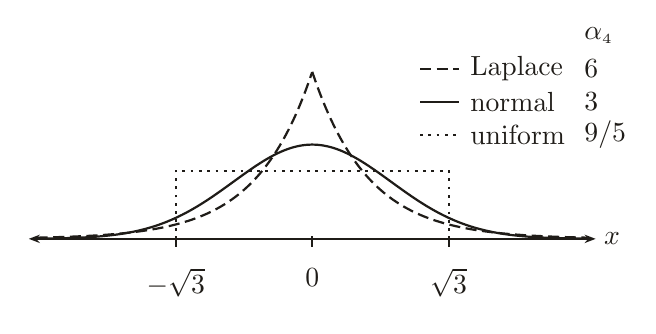
\begin{tikzpicture}[
  x=1cm,
  y=3cm,
  every node/.style={font=\normalsize, journalink},
  axis/.style={journalink, line width=0.8pt,
               {Stealth[length=4pt]}-{Stealth[length=4pt]}},
  tick/.style={journalink, line width=0.8pt},
  normalcurve/.style={journalink, line width=0.8pt},
  laplacecurve/.style={journalink, line width=0.8pt,
               dash pattern=on 4pt off 2pt},
  uniformcurve/.style={journalink, line width=0.8pt,
               dash pattern=on 1pt off 2pt}
]
  % ---- the three densities --------------------------------------------
  % N(0,1), solid, the reference peak
  \draw[normalcurve] plot[domain=-3.5:3.5, samples=300, smooth]
    (\x,{0.3989423*exp(-\x*\x/2)});

  % Laplace, mean 0 and variance 1: b = 1/sqrt(2).  Drawn as two halves so
  % that the corner at x = 0 stays a corner and is not rounded by smooth.
  \draw[laplacecurve] plot[domain=-3.5:0, samples=200, smooth]
    (\x,{0.7071068*exp(1.4142136*\x)});
  \draw[laplacecurve] plot[domain=0:3.5, samples=200, smooth]
    (\x,{0.7071068*exp(-1.4142136*\x)});

  % U(-sqrt3, sqrt3): the density is positive on that interval only, so the
  % two ends drop to the axis.
  \draw[uniformcurve] (-1.7320508,0) -- (-1.7320508,0.2886751)
    -- (1.7320508,0.2886751) -- (1.7320508,0);

  % ---- x axis ----------------------------------------------------------
  \draw[axis] (-3.6,0) -- (3.6,0);
  \node[anchor=west, inner sep=2.8pt] at (3.6,0) {$x$};

  \foreach \p in {-1.7320508, 0, 1.7320508}
    \draw[tick] ([yshift=0.035cm]\p,0) -- ([yshift=-0.106cm]\p,0);
  \node[anchor=north] at ([yshift=-0.25cm]-1.7320508,0) {$-\sqrt{3}$};
  \node[anchor=north] at ([yshift=-0.25cm]0,0) {$0$};
  \node[anchor=north] at ([yshift=-0.25cm]1.7320508,0) {$\sqrt{3}$};

  % ---- legend, top right corner ---------------------------------------
  % Sample segments 0.5cm long per spec 1.9, from x = 1.37 to x = 1.87.
  % 2026-08-13: the author asked twice for the legend to move right; it was
  % reading as cramped against the curves on its left.  The whole block was
  % shifted right by 0.85cm, which is the largest shift that keeps the
  % drawing's bounding box at 219.951 units wide.  Beyond that the legend,
  % rather than the x-axis label, sets the right edge and the whole figure
  % grows (0.95cm widens it to 222.204, 1.00cm to 223.622), which would
  % shrink every glyph by the same ratio once the SVG is fitted to 350px.
  % Rows at 2.58 / 2.16 / 1.74 / 1.32 cm above the axis: the lowest of them
  % clears the Laplace curve, which reaches 1.32cm at |x| = 0.335, by
  % 0.185cm, and the head row stands 0.46cm above the Laplace peak.
  \node[anchor=west, inner sep=0pt] at ([yshift=2.58cm]3.45,0)
    {$\alpha_{\sssig 4}$};

  \draw[laplacecurve] ([yshift=2.16cm]1.37,0) -- ([yshift=2.16cm]1.87,0);
  \node[anchor=west, inner sep=0pt] at ([yshift=2.16cm]2.00,0) {Laplace};
  \node[anchor=west, inner sep=0pt] at ([yshift=2.16cm]3.45,0) {$6$};

  \draw[normalcurve] ([yshift=1.74cm]1.37,0) -- ([yshift=1.74cm]1.87,0);
  \node[anchor=west, inner sep=0pt] at ([yshift=1.74cm]2.00,0) {normal};
  \node[anchor=west, inner sep=0pt] at ([yshift=1.74cm]3.45,0) {$3$};

  \draw[uniformcurve] ([yshift=1.32cm]1.37,0) -- ([yshift=1.32cm]1.87,0);
  \node[anchor=west, inner sep=0pt] at ([yshift=1.32cm]2.00,0) {uniform};
  \node[anchor=west, inner sep=0pt] at ([yshift=1.32cm]3.45,0) {$9/5$};
\end{tikzpicture}
\end{document}
